% =====================================================================================
% COMPUTATIONAL METHODS.
% SOURCES OF NUMBERS (PaperData = /home/Ubuntu/PaperRuns/PaperData):
%   DFT, data, NEP ........ PaperData/Task2_DFTcampaign, Task3_MLFF*, plan-docs/Task1_configuration_generation_plan.md
%   MD protocol ........... PaperData/Task4_PhaseTransition/README.md, make_size.py, make_stress.py,
%                           size_A_*/inputs/simParameters.json, stress_A_*/inputs/simParameters.json
%   P_ext values .......... DFTengine/r2scan_bugfix_work/pulay/pulay.md
%   Phase identification .. Task4_PhaseTransition/d3_compare.py, size_compare.md, README.md (PDynA checks)
%   Band-gap estimators ... Task4_PhaseTransition/select_gap_frames.py, gap_estimate.py, dft_gap/README.md
% Do not add a number that is not in those files; use \todo{} instead.
% =====================================================================================

\subsection{Overview}
\label{sec:overview}

The workflow has four parts (Figure~\ref{fig:workflow}). First, a broad pool of
configurations of the three compounds is generated by MD with an existing force
field and down-sampled to a training set, which is labelled with DFT. Second, machine-learned
potentials are fine-tuned on these labels and validated against held-out DFT data and
against DFT calculations on configurations from its own MD. Third, UrsaMLFF
drives large-scale MD: heating and cooling ramps locate the transition
temperatures of the free-standing crystals, and anneal-and-cooling runs
under two substrate constraints and without one describe a clamped
film. Fourth, frames of these ensembles are selected by stratified sampling
and their band gaps are computed with DFT. Every quantity reported as a result
is a difference between two matched states.

\begin{figure}[htbp]
  \centering
  \resizebox{\linewidth}{!}{%
  \begin{tikzpicture}[node distance=5mm,
      box/.style={draw, rounded corners=2pt, align=center, font=\footnotesize, text width=38mm,
                  minimum height=37mm, inner sep=3pt,
                  execute at begin node={\hyphenpenalty=10000\exhyphenpenalty=10000}},
      arr/.style={-{Stealth[length=2mm]}, thick}]
    \node[box] (a) {\textbf{Configuration generation}\\[3pt] (i)Sampling MD of all phases,\\ strains and cation orders\\[2pt]
      (ii) Selection by atomic environment coverage\\ in latent space\\[2pt] (iii)DFT labeling\\ (PBEsol, \rSCAN{})};
    \node[box, right=of a] (b) {\textbf{Force fields}\\[3pt] fine-tuning of\\ UrsaMLFF and MACE\\[2pt]
      held-out and\\ out-of-distribution\\ DFT tests};
    \node[box, right=of b] (c) {\textbf{Molecular dynamics}\\[3pt] heating and cooling ramps,\\ cell-size convergence,\\
      transition temperatures\\[2pt] anchored clamping study:\\ free, stress-controlled,\\ rigid clamp};
    \node[box, right=of c] (d) {\textbf{Band gaps}\\[3pt] stratified selection\\ of MD frames\\[2pt]
      DFT on complete\\ production frames\\[2pt] paired and\\ ensemble \dEg{}};
    \draw[arr] (a) -- (b);
    \draw[arr] (b) -- (c);
    \draw[arr] (c) -- (d);
  \end{tikzpicture}}
  \caption{Workflow: configuration generation and DFT labelling, fine-tuning
    and validation of the force fields, MD of free-standing and clamped cells, and stratified DFT
    band gaps of selected MD frames.}
  \label{fig:workflow}
\end{figure}

% 2026-10-29 (user): methods condensed; the details moved to the Supporting Information (si/si_body.tex sections
% si:dftconv, si:ff, si:models; si/configurationGeneration.tex). Previous version: git history.
\subsection{Electronic structure}
\label{sec:dft}

{\changedcolor
The energies, forces and stresses used to train the force fields, and the band gaps of selected MD frames, are
obtained from Kohn--Sham density functional theory (DFT) with our in-house code UrsaDFT. The Kohn--Sham equations may
be discretised in any complete basis, such as finite elements or plane waves; here we employ plane waves together with
Bl\"ochl's projector augmented-wave (PAW) method\cite{Blochl1994PAW} and the JTH PAW datasets
(version~2.0),\cite{Jollet2014CPC, JTHv2web} which are generated with the PBE functional. Exchange and correlation are
treated at two levels of approximation for both the labels and the band gaps: the generalised-gradient approximation
(GGA) with PBEsol\cite{Perdew2008PBEsol} and the meta-GGA with \rSCAN{}.\cite{Furness2020r2SCAN} The \rSCAN{}
meta-GGA proved more robust and accounts for most of the experimental observations
(\emph{Choice of the exchange--correlation functional}). The main text therefore reports \rSCAN{} results, including the MD of the
clamping study (\emph{Effect of process conditions on band-gap deviations}), with the band gaps of the hybrids; the band gaps of \CsSnI{} in that study are those of the earlier PBEsol study. The remaining PBEsol results are given
in the Supporting Information. Spin--orbit coupling is neglected throughout. The plane-wave cutoffs were chosen such
that the discretisation errors remain below \SI{2e-4}{\hartree} per atom in the energy,
\SI{2e-4}{\hartree\per\bohr} in the forces and \SI{5e-6}{\hartree\per\bohr\cubed} in the stress; further details are
given in the Supporting Information.
}

\subsection{Identifying structures for DFT labelling}
\label{sec:data}

{\changedcolor
The structures labelled with DFT are drawn from MD trajectories that span, with margin, every state the production
simulations visit: the $\alpha$, $\beta$ and $\gamma$ phases and the transitions between them, the strains of thermal
expansion, of the transitions and of substrate clamping, and disordered orientations of the molecular cations. With
the UrsaMLFF foundation model we ran constant-volume and constant-pressure simulations of the phases of \CsSnI{},
\MASnI{} and \FASnI{}. The starting structures were the three phases of each compound built from their Glazer tilt
patterns,\cite{Glazer1972} structures from the Materials Project,\cite{mp2013} and frameworks of documented Pb-based
perovskites in which Pb was replaced by Sn (Table~\ref{tab:mp}). The foundation model only proposes structures, since
every selected structure is recomputed with DFT. The trajectories form a pool of \num{55928} structures (Supporting
Information).

Our workflow then identifies the distinct atomic environments of the pool and selects the structures that cover all
of them at the lowest DFT cost. Every atom is described by Gaussian multipole descriptors;\cite{Lei2019GMP, Lei2022GMP}
environments closer than a cutoff in this descriptor space are treated as equivalent, which leaves 3816 distinct
environments, and a greedy set cover weighted by the cell volume selects the cheapest set of structures that contains
all of them. Together with one structure from each sampling stratum that the cover missed and a second round of small
structures, 718 structures of 36 to 432 atoms were labelled: 320 of \MASnI{}, 247 of \FASnI{}, 136 of \CsSnI{} and 15
of reference compounds.

Large-scale MD with the first potentials revealed configurations that these labels do not cover and in which the
force field failed: protons detached from their cation, broken C--N bonds and two cations in one cage in the hybrids,
and Cs ions passing into a neighbouring cage in \CsSnI{}. Such configurations were labelled in an active-learning
loop: cells cut around the defect events of the MD, images in which an N--H or C--H bond is stretched or a Cs--Sn,
C--I, N--I or H--I contact is shortened, and frames of the hottest MD. Table~\ref{tab:labels} gives the tally of the
DFT labels; the details are given in the Supporting Information.
}

\begin{table}[htbp]
  \centering
  \caption{\changed{DFT labels of this work. Initial: structures selected from the sampling pool; active learning:
    structures added after failures of the force field in large-scale MD; used: training, validation and held-out
    structures after the exclusions given in the Supporting Information.}}
  \label{tab:labels}
  \begin{tabular}{lrr}
    \toprule
    & PBEsol & \rSCAN{} \\
    \midrule
    initial selection & 718 & 721 \\
    active learning: molecular defects & 212 & 205 \\
    active learning: Cs--Sn, C--I, N--I and H--I contacts, hot MD & -- & 120 \\
    \midrule
    total computed & 930 & 1046 \\
    \bottomrule
  \end{tabular}
\end{table}

\subsection{Fine-tuning the machine-learned potentials}
\label{sec:nep}

{\changedcolor
We fine-tune two classes of machine-learned interatomic potentials on the labels of each functional. The first is the
equivariant message-passing MACE architecture,\cite{Batatia2022MACE} initialised from the foundation models
MACE-MH-1\cite{MACEMH1} and MACE-OMAT-0-medium.\cite{ref_mace_omat, Batatia2023Foundation} The second is our in-house
force field UrsaMLFF, whose radial and angular descriptors and per-element networks follow
refs~\citenum{ref_nep} and~\citenum{Song2024NEP4}, extended by one equivariant message-passing step. UrsaMLFF carries
all production MD, as it is fast enough for nanosecond trajectories of cells with thousands of atoms; the more accurate
but slower MACE models serve to validate it. The potentials are fitted to cohesive energies, forces and the full stress
tensor. The labelled structures are divided by MD trajectory, and stratified by compound, into training, validation and
held-out sets; the final UrsaMLFF is trained on the complete \rSCAN{} training set of 866 structures, including the
active-learning labels. Architectures and training settings are given in the Supporting Information.

Table~\ref{tab:holdout} and Figure~\ref{fig:parity} report the accuracy of the \rSCAN{} potentials on the held-out
structures. All three reproduce the DFT forces with $R^2 \ge 0.99$ and the energies within a compound with
$R^2 \ge 0.98$. The MACE models predict forces about twice as accurately as UrsaMLFF, whereas UrsaMLFF predicts
stresses 2.3 to 4.7 times more accurately, the stress error of the MACE models being dominated by a constant pressure
offset. On a single A100 GPU, UrsaMLFF performs 960 to 2540 MD steps per second for cells of up to 2300 atoms, 70 to
135 times more than the faster MACE model. Dispersion is included at run time through Grimme's D3 correction with
Becke--Johnson damping\cite{Grimme2010D3, Grimme2011BJ} and the parameters of the training functional; it is not part
of the fit. The PBEsol potentials and the throughput benchmark are reported in the Supporting Information.
}

% generated by PaperData/paper_figs/fig_holdout.py; do not edit
\begin{table}[htbp]
\centering
\caption{Errors of the potentials trained on the \rSCAN{} labels on the 99 held-out structures: root-mean-square errors of the energy per atom, the force components and the stress components, and coefficients of determination $R^2$ (for the energy after subtracting the mean DFT energy of each compound). \changed{UrsaMLFF: final potential, trained on 866 structures including the active-learning labels; MACE: fine-tuned on the 546 initial structures.}}
\label{tab:holdout}
\resizebox{\linewidth}{!}{%
\begin{tabular}{lcccccc}
\toprule
model & $E$ (\si{\hartree}/atom) & $F$ (\si{\hartree\per\bohr}) & $\sigma$ (\si{\hartree\per\bohr\cubed}) & $R^2_E$ & $R^2_F$ & $R^2_\sigma$ \\
\midrule
\changed{UrsaMLFF} & \changed{\num{9.23e-5}} & \changed{\num{5.20e-4}} & \changed{\num{8.51e-7}} & \changed{0.9865} & \changed{0.9986} & \changed{0.9974} \\
MACE-MH-1 & \num{4.37e-5} & \num{2.48e-4} & \num{4.01e-6} & 0.9970 & 0.9997 & 0.9429 \\
MACE-OMAT & \num{9.78e-5} & \num{2.67e-4} & \num{1.99e-6} & 0.9848 & 0.9996 & 0.9860 \\
\bottomrule
\end{tabular}}
\end{table}


\begin{figure}[htbp]
  \centering
  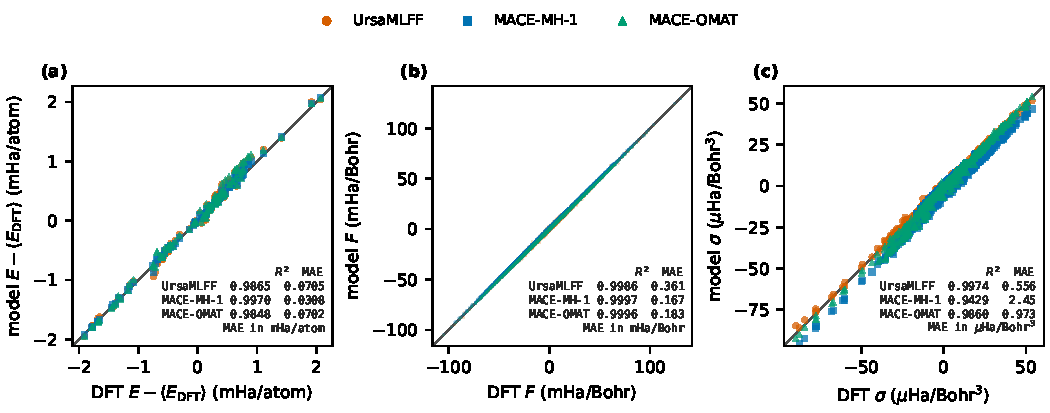
\includegraphics[width=\linewidth]{figures/fig_parity.pdf}
  \caption{\changed{Predicted against DFT values on the 99 held-out structures for the potentials trained on the
    \rSCAN{} labels: (a) energy per atom relative to the mean DFT energy of each compound, (b) force components,
    (c) stress components. Insets: coefficient of determination $R^2$ and mean absolute error (MAE) of each potential.}}
  \label{fig:parity}
\end{figure}

\subsection{Molecular dynamics}
\label{sec:md}

{\changedcolor
MD is run with the GPU engine of UrsaMLFF in double precision. Temperature is controlled by stochastic velocity
rescaling\cite{Bussi2007JCP} and pressure by stochastic cell rescaling,\cite{Bernetti2020JCP} with the three orthogonal
cell axes coupled independently and an external pressure that offsets the Pulay stress of the labels. All cells are
supercells of the orthogonal $\sqrt{2}\times\sqrt{2}\times2$ setting of the cubic perovskite, in which the cubic,
tetragonal ($P4/mbm$, $I4/mcm$) and orthorhombic ($Pnma$) phases are all orthogonal, so every transition can proceed
by rescaling the three axes, without shear. The production cells contain 2000 atoms for \CsSnI{} and 2304 atoms for
\MASnI{} and \FASnI{}. Transitions are located with linear temperature ramps at constant pressure at \SI{0.25}{K/ps}.
Each compound is cooled from the cubic phase, from 450 to \SI{500}{K} (\CsSnI{}) or \SI{400}{K} (hybrids) down to
\SI{200}{K} or \SI{50}{K}, and the cooled crystal is heated back over the same range at the same rate. \MASnI{} is also heated from an in-phase tilted crystal to test the role of the thermal path. Every protocol is run
three times with different initial velocities. Ramps of 0.1 to \SI{2}{K/ps} and cells of up to \num{23040} atoms,
given in the Supporting Information, show how the transition temperatures depend on rate and cell size.
% rate/size studies: si/tab_rates and si/tab_20k (v2r2c, 2026-10-29); si/tab_size still v2r2al (2 K/ps size series)
\apc{} denotes the cube root of the volume per formula unit. Ensembles, starting structures and run parameters are
given in the Supporting Information.
}

\subsection{Phase identification and transition temperatures}
\label{sec:phaseid}

{\changedcolor
We analyse the octahedral tilts in the MD trajectories with PDynA.\cite{Liang2023PDynA} For every frame, PDynA computes
the tilt angles of every SnI$_6$ octahedron about the three pseudo-cubic axes and the correlation between the tilts of
nearest-neighbour octahedra along each axis. The sign of this correlation distinguishes in-phase ($+$) from antiphase
($-$) tilting and so identifies the Glazer tilt pattern.\cite{Glazer1972} The correlations are averaged over all
octahedra and over \SI{10}{K} windows of the heating and cooling ramps. The phases and transition temperatures are then
assigned from the loss of tilt order, with the criteria of Table~\ref{tab:phaseid}. Because the order parameters are the
absolute correlations sorted by size, the assignment does not depend on which cell axis carries which tilt, which a
cooling run chooses at random. The low-temperature phase of \FASnI{} ($P4bm$) adds no tilted axis but alternates the tilt
amplitude between successive layers; we detect it with the layer alternation $S$, half the difference between the mean
rms tilts of even and odd layers about the tilt axis in \SI{14}{ps} time averages, computed every \SI{10}{K}.
}

\begin{table}[htbp]
  \centering
  \caption{\changed{Assignment of phases and transitions from the nearest-neighbour tilt correlations $C_a$, $C_b$ and
    $C_c$ about the three pseudo-cubic axes (degrees), averaged over all octahedra in windows of \SI{10}{K} spaced by
    \SI{5}{K}. $|C|_{(1)} \geq |C|_{(2)} \geq |C|_{(3)}$ are the absolute correlations sorted by size; $\alpha$: cubic, $\beta$: tetragonal,
    $\gamma$: orthorhombic. The thresholds
    are at least twice the values in the phase above the transition. A transition temperature is the hottest window of an ordered
    stretch of at least \SI{20}{K} (three consecutive windows above the threshold); we report the mean and standard
    error over the runs, on cooling and on heating.}}
  \label{tab:phaseid}
  \small
  \begin{tabular}{llll}
    \toprule
    & order parameter & criterion & compounds \\
    \midrule
    tilt sense & $C$ about the tilted axis & $+$ in-phase, $-$ antiphase & all \\
    $\beta\leftrightarrow\alpha$ transition & $|C|_{(1)}$, any tilt & falls below \ang{3} & all \\
    $\gamma\leftrightarrow\beta$ transition & $|C|_{(2)}$, second tilted axis & falls below \ang{2}
      & \CsSnI{}, \MASnI{} \\
    layered tilt ($P4bm$) & $S$, layer alternation & falls below \ang{1} & \FASnI{} \\
    \bottomrule
  \end{tabular}
\end{table}


\subsection{\protect\changed{Free energy of the tilt sense}}
\label{sec:ti}
% Sources (2026-10-29): PaperData/Task4_PhaseTransition/tilt_sense/ti_free: make_r2lat_structs.py (cells), ti_md2.py
% (--set r2), make_ti2_jobs.py, ti2_node.sh, ti_analyze2.py (TI_SET), r2_summaries/; a100-7 ~/ti_free/out2_r2 (91 windows).
% 2026-10-30: with D3 (ti_md2.py --d3): sets r2d3 (FASnI3 restarts), r2d3s (MASnI3 from scratch), pbd3 (PBEsol, own
% lattice); d3_summaries/ti2_summary_<set>.json (a100-1 ~/ti_ana); SI table si/tab_ti_xc.tex (paper_figs/tab_ti_si.py).
{\changedcolor
The free-energy difference between the antiphase and the in-phase tilt is computed by thermodynamic
integration\cite{Kirkwood1935JCP} in fixed tilted frameworks, in which only the cations move. The cells contain 128
formula units (1536 atoms, $4\times4\times2$ repeats of the $\sqrt{2}\times\sqrt{2}\times2$ setting) with the volume of
the force field at \SI{200}{K}, a cubic metric of \SI{6.292}{\angstrom} for \FASnI{} and \SI{6.237}{\angstrom} for
\MASnI{}. The octahedra are rotated about $c$ by the experimental tetragonal tilt (Table~\ref{tab:expt-tilt}), \ang{6.3}
for \FASnI{} and \ang{8.6} for \MASnI{}, in phase ($a^0a^0c^+$) or in antiphase ($a^0a^0c^-$). The two frameworks share
the Sn atoms, the axial I atoms and the equatorial I atoms of every second layer, and differ only in the equatorial I
atoms of the other layers, whose rotation is reversed. These atoms are moved along the straight path
$\mathbf{x}(\lambda) = \mathbf{x}_{+} + \lambda(\mathbf{x}_{-} - \mathbf{x}_{+})$ from the in-phase ($\lambda = 0$) to
the antiphase framework ($\lambda = 1$), and
\begin{equation}
  \Delta F = F_{-} - F_{+} = \int_0^1 \left\langle \frac{\partial U}{\partial\lambda} \right\rangle_\lambda \mathrm{d}\lambda ,
  \qquad
  \frac{\partial U}{\partial\lambda} = -\sum_i \mathbf{F}_i \cdot (\mathbf{x}_{-,i} - \mathbf{x}_{+,i}) ,
\end{equation}
where the sum runs over the moving I atoms and $\mathbf{F}_i$ are the forces on them. Because the framework is held
fixed, $\Delta F$ isolates the contribution of the cations, through their orientations and their contacts with the
iodide cage; a positive $\Delta F$ favours the in-phase tilt.

The cations are propagated at constant volume with stochastic velocity rescaling (time step \SI{1}{fs}, time constant
\SI{100}{fs}), with D3 added to every energy and force. Each window starts from a random orientation of every cation,
the same in both frameworks, is held for \SI{20}{ps} at \SI{350}{K}, and is then cooled to 300, 250 and \SI{200}{K},
with \SI{20}{ps} of equilibration and \SI{100}{ps} of production at each temperature. For \FASnI{}, the windows
instead continue those of a first calculation without D3, which was cooled in steps of \SI{25}{K} from 325 to
\SI{100}{K}: from its configurations at 200 and \SI{300}{K}, each window is run with D3 for \SI{20}{ps} of
equilibration and \SI{100}{ps} of production. The calculation without D3 gives the temperature dependence over the
wider range (Supporting Information). The integrand is sampled at the nine Gauss--Lobatto nodes of $\lambda$, with five further windows
between $\lambda = 0.75$ and 0.97 for \FASnI{}, where it changes rapidly, and integrated by Gauss--Lobatto quadrature;
as an independent estimate, the potential energy of each configuration is evaluated every \SI{1}{ps} at every
$\lambda$ of the path and $\Delta F$ is obtained with MBAR.\cite{Shirts2008JCP} The energy difference follows from the
end windows, $\Delta U = \langle U\rangle_{-} - \langle U\rangle_{+}$, and the entropic part as
$-T\Delta S = \Delta F - \Delta U$. Every calculation is repeated for three independent cation arrangements (six for
\MASnI{} at \ang{8.6}), and we report the mean and standard error. The same calculations are made with the PBEsol
potential and D3, at the volume of that potential at \SI{200}{K} (\SI{6.116}{\angstrom} for \FASnI{} and
\SI{6.079}{\angstrom} for \MASnI{}). For \MASnI{}, both potentials are also evaluated at a tilt of \ang{4}, and with
the framework atoms tethered to their positions by springs of \SI{0.031}{\hartree\per\bohr\squared} instead of being
fixed, to test the rigid framework. For \FASnI{}, the windows above $\lambda = 0.84$ are repeated from the configuration
equilibrated at $\lambda = 0.84$, to test for hysteresis along the path, and the two end states at $\lambda = 1$ are
joined in one cell (half of each) to test which cation arrangement is stable in the antiphase framework.
}
